\section{Core Java}

The first section deals with Java primitives, objects and their life cycle, and some JDK-provided classes for String manipulation and Collections. It includes writing applications to sort Strings. It also deals with Exceptions and Enums.

\subsection{Object Life cycle}
\begin{center}\textit{Describe the life cycle of an object instance in Java and how garbage collection works}\end{center}

\paragraph{Procedural programming preceded object-oriented programming.} Basically, The code was written line by line, like a recipe. The computer would execute the lines in the order they appeared in the program. There were constructs to jump from one place to another, called gotos. But very quickly a program can become quite complicated, and specially the gotos would make it very hard to follow. 

With many lines of code, the program becames difficult to maintain. We can split the program into several files and import the pieces when compiling. That helps humans to organize the data but also fulfills the need for the compiler to have all the pieces of the program available. It doesn't solve the problem of scope, though. In procedural programming the data is accessible to the entire program. There is no clear ownership of data.

Procedural programming also provided constructs called subroutines. They are blocks of code, collections of instructions. Subroutines have their own scope, but any data they need to access outside the subroutine is still exposed to the entire program.

\begin{figure*}[ht]\centering % Using \begin{figure*} makes the figure take up the entire width of the page
\includegraphics[width=\linewidth]{object-life-cycle}
\caption{Object Life Cycle}
\label{fig:object-life-cycle}
\end{figure*}

\paragraph{Java is an object-oriented language.} In object-oriented languages, instead of having data and subroutines, we deal with objects that have data and behavior. WIth object-oriented programming we can easily model the real world. For example we can have an object of a dog that has data (color, breed) and behavior (barks, runs, drools). 

When developers write java programs, they write classes. A class is like a blueprint of an object, it defines the object. A class becomes an object when we instanciate it, we create an instance of it. Obects live when the program is executing, at runtime.

With objects it is easy to encapsulate behavior and data. We can restrict access to the data to only the members inside of a class. Nobody outside the class can access the data, if we don't want to ( and we shouldn't want to.) We can define interfaces that provide indirect, controlled access to the data inside the class.

Organizing code becomes easier too, because each file can only have one  public class per file. Since each class encapsulate one "thing", that has a well-defined interface that determines its behaviors, the code becomes very logical.

Everything in Java is made of another object. We call this inheritance. Java provides the mother of all objects, called \texttt{Object}, from which any other class must inherit.

\paragraph{Instantiating a class.} We create an object from a class with the Java keyword \texttt{new}. Before instantiation, the object doesn't exist. After instantiation it exists. Classes have a special method called a constructor. After creating the class the Java Virtual machine (JVM) calls the object's constructor. If you don't provide a constructor for your class, the its parent (eventually the \texttt{Object} constructor is called. The constructor is a place where you coudl initialize the object or start resources.\cite{nicholas}

\paragraph{Strongly Referenced.} When the constructor has been called, your program has a strong reference to it.\cite{reference} It means you can access the non-private methods and data on it. It is usable by your program.
\begin{lstlisting}[language=Java]
Dog pepper = new Dog();
\end{lstlisting}
In the above example, \texttt{pepper} is the handle to your object, or a reference. It is a strong reference (as opposed to a weak reference) because you can use it to do things with the \texttt{pepper} object:
\begin{lstlisting}[language=Java]
pepper.bark();
\end{lstlisting}

You can have several references to the same object:
\begin{lstlisting}[language=Java]
// create an instance of Dog
Dog pepper = new Dog();

// pepperClone also points to the same object
pepperClone = pepper;

// set pepper's name to "pepper"
pepper.setName("pepper");

// returns "pepper"
pepperClone.getName();

\end{lstlisting}
In the above example we created an instance of a \texttt{Dog} and got back a reference to it called \texttt{pepper}. Then we made \texttt{pepperClone} also point to the same object. After that we set the name of \texttt{pepper} to "pepper". Because \texttt{pepper} and \texttt{pepperClone} point to the exact same object, when we ask \texttt{pepperClone} for its name, we get "pepper".

\begin{figure}[H]\centering % Using \begin{figure*} makes the figure take up the entire width of the page
\includegraphics[width=0.5\linewidth]{object-reference}
\caption{Object References}
\label{fig:object-references}
\end{figure}
\paragraph{Other references.} Once you let go of all the references to an object, it becomes eligible for garbage collection. The JVM still holds a weak or soft reference to the object (so it can manage it), but eventually, when it detects that memory needs to be cleaned up, it will finalize the object.\cite{reference}

\paragraph{Garbage Collection.} When the JVM determines that it needs to free memory, it will perform a garbage collection. The soft and weak references will be cleared before throwing an \texttt{OutOfMemoryException}. 

Garbage collection is controlled by the JVM. There are tweaks you can do to suggest a certain behavior to the garbage collector, and you can even suggest that it will do garbage collection (generally not a good idea), but eventually the garbage collector will decide when to run.

The benefit of garbage colection is that the programmer doesn't need to think about finalizing objects. When they are not needed, they may be thrown into garbage automatically. There are times when this thinking can get you into troublem though. If you don't release the references the objects will never be garbage collected. An object is released when the program no longer holds a reference to it. You can either set the reference to null or it will automatically be released when your object goes out of scope.
\begin{figure}[H]\centering % Using \begin{figure*} makes the figure take up the entire width of the page
\includegraphics[width=\linewidth]{garbage-collection}
\caption{Garbage Collection}
\label{fig:garbage-collection}
\end{figure}
The above image shows garbage collection in action. I wrote a little program that creates objects and puts them in a collection. I used the visualvm tool provided in the Oracle JDK distribution\cite{garbagecollection}. After every 10000 objects I clear the collection. I wrote created a total of 306,480,000 objects, so I cleared the collection over 30,000 times. Garbage collection, though only kicked in 7 times. I had set my heap size to 25MB. 

In the image you can also see the movement of objects from one generation to another.


\subsection{Basic Data Types}
\textit{Describe how the basic data types are represented in memory (boolean, int, long, String, array of ints, array of Objects, class with fields)}
\paragraph{Java's primitive types} can be divided into two\footnote{Really, there are three. The third one, \texttt{returnAddress}, is not available for the programmer} main groups: numeric primitives, and boolean. Numeric primitives consist of integral and floating point primitives.\cite{gosling}

\begin{figure}[H]\centering
\includegraphics[width=\linewidth]{primitives}
\caption{Primitive Classification}
\label{fig:results}
\end{figure}

Java specification\cite{gosling} defines sizes and ranges for primitive types. The integer types are clear cut, but the floating point types are not so simple. They follow the ANSI/IEEE Standard 754-1985\footnote{see http://docs.oracle.com/javase/specs/jls/se7/html/jls-4.html\#jls-4.2.3 for details}. The values in table~\ref{tab:java-primitive-types} are from my MacBookPro, printing out the max value for float and double. They might be different on a different architecture.

Also to note that although Java defines the primitive sizes, on different architectures might actually use different sizes. For example, although an int is defined as 32 bits, it might take 64 bits on a 64 bit computer. The primitive sizes defined in the Java Specification is how the programmer sees the types, not necessarily how they are stored.

The list of primitives in Java\cite{gosling}:
\begin{table}[!htb]
\centering
\begin{tabulary}{\columnwidth}{ | p{0.1\columnwidth} | p{0.15\columnwidth} | p{0.55\columnwidth} |}
\hline
\textbf{Type} & \textbf{Size (bits)} & \textbf{Range} \\ \hline 
byte  & 8  & from -128 to 127, inclusive \\ \hline 
short & 16 & from -32768 to 32767, inclusive \\ \hline 
int   & 32 & from -2147483648 to 2147483647, inclusive \\ \hline 
long  & 64 & from -9223372036854775808 to 9223372036854775807, inclusive \\ \hline
char  & 16 & from '\textbackslash{}u0000' to '\textbackslash{}uffff' inclusive, that is, from 0 to 65535 \\ \hline 
float & 32 & from -3.4028235E38 to 3.4028235E38\footnotemark[3] \\ \hline
double & 64 &from -1.7976931348623157E308 to 1.7976931348623157E308\footnotemark[3] \\ \hline
boolean & 32\footnotemark[4] & true or false \\ \hline
\end{tabulary}
\caption{Java Primitive Types}\label{tab:java-primitive-types}
\end{table}

\footnotetext[3]{Java float and double follow the  ANSI/IEEE Standard 754-1985, see http://docs.oracle.com/javase/specs/jls/se7/html/jls-4.html\#jls-4.2.3}
\footnotetext[4]{\texttt{boolean} is internally implemented like an \texttt{int}}
[TODO: How are the primitives stored (heap, stack)]
\paragraph{class with fields}
[TODO: How are the classes stored (heap, stack)]
\paragraph{String} in Java is represented by sequences of Unicode code points. String is a sequence of characters, which each is represented by two bytes. 
[TODO: How are the strings stored (heap, stack)]
\paragraph{array of ints}
[TODO: How are the array of ints stored (heap, stack)]
\paragraph{array of Objects}
[TODO: How are the array of objects stored (heap, stack)]

%------------------------------------------------

\subsection{List of Strings}
\textit{Write an application to find out how many total characters can be held in a list of strings before you run out of memory}

some text



\subsection{StringBuffer vs StringBuilder}
\textit{Compare and contrast StringBuffer and StringBuilder and when to use each}
Notes: What does it mean to be concurrency resistant? Example? write sample application to show concurrent insert and non concurrent. Check for execution times. show concurrency failure. string+ is actually a better comparison point (who writes to strings from different threads?)

StringBuffer is designed to be thread-safe and all public methods in StringBuffer are synchronized. StringBuilder does not handle thread-safety issue and none of its methods is synchronized.

http://stackoverflow.com/questions/16653119/imagine-a-real-concurrent-scenario-where-stringbuffer-should-be-used-than-string (last examnple) Test with aaaaaa and bbbb strings of equal length, or different lengths.


\begin{figure}[H]\centering
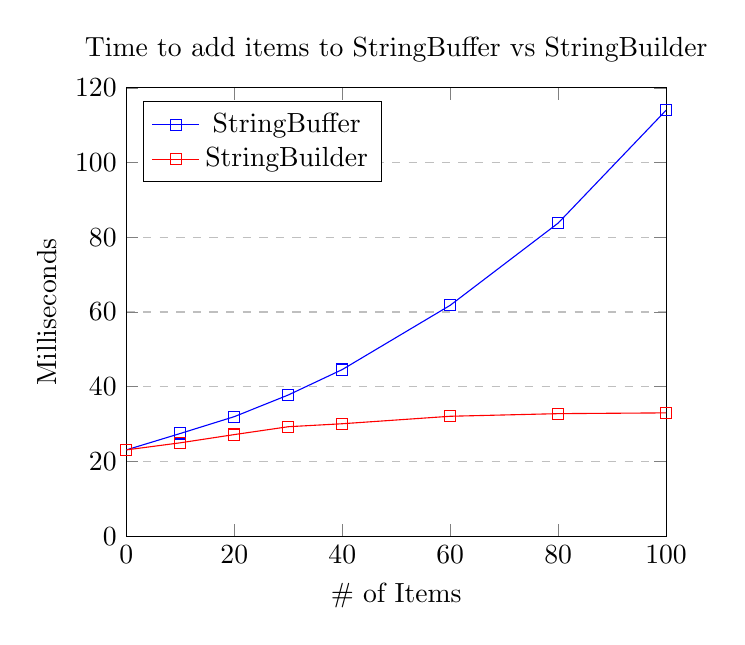
\begin{tikzpicture}
\begin{axis}[
    title={Time to add items to StringBuffer vs StringBuilder},
    xlabel={\# of Items},
    ylabel={Milliseconds},
    xmin=0, xmax=100,
    ymin=0, ymax=120,
    xtick={0,20,40,60,80,100},
    ytick={0,20,40,60,80,100,120},
    legend pos=north west,
    ymajorgrids=true,
    grid style=dashed,
]
% StringBuffer
\addplot[
    color=blue,
    mark=square,
    ]
    coordinates {
    (0,23.1)(10,27.5)(20,32)(30,37.8)(40,44.6)(60,61.8)(80,83.8)(100,114)
    };
% StringBuilder
\addplot[
    color=red,
    mark=square,
    ]
    coordinates {
    (0,23.1)(10,25)(20,27.2)(30,29.3)(40,30.1)(60,32.1)(80,32.8)(100,33.01)
    };
    \legend{StringBuffer, StringBuilder}
 
\end{axis}
\end{tikzpicture}\caption{Insert time into a StringBuilder vs. a StringBuffer}
\label{fig:stringbuildervsStringBuffer}
\end{figure}

Reference to Figure \ref{fig:results}.


\subsection{Collections}
\textit{Compare/contrast use of ArrayList / LinkedList / HashMap / HashSet / TreeSet}
Notes: write sample application to show the use of the collections. Check for execution times
Make a table for comparison

some text

\subsection{Sorting in Order}
\textit{Write an application to read a file with 10k lines of text, and output another file with the lines in sorted order.}

some text

\subsection{Sorting in Reverse Order}
\textit{Write an application to read a file with 10k lines of text, and output another file with the lines in reverse sorted order}

some text


\subsection{Exceptions}
\textit{Write code to show exception handling including examples of checked, unchecked, and Error exceptions}

some text

\subsection{Enums}
\textit{Write your own enum type.  Describe when you would use it.}

some text
